\documentclass[10pt]{article}
\usepackage[top=1in, bottom=1in, left=1in, right=1in]{geometry}
\usepackage{float}
\usepackage{color}
\usepackage{picture}
\usepackage{listings}
\usepackage{caption}
\usepackage{hyperref}
\usepackage{graphicx}
\usepackage{amsmath}
\usepackage{subcaption}
\usepackage[utf8]{inputenc}

% Used to change font to Times TX
\usepackage{txfonts}
\usepackage[T1]{fontenc}

% Used for the figures that have been inserted into the document.
\floatstyle{plain} 
\restylefloat{figure}

% Used so as not to indent paragraphs.
\setlength\parindent{0pt}

% Used for syntax highlighting in code.
\definecolor{skyblue}{rgb}{0.53, 0.81, 0.92}
\definecolor{lightred}{rgb}{0.90, 0.36, 0.36}
\definecolor{darkkhaki}{rgb}{0.71, 0.51, 0.06}

% Default parameters for listings package.
\lstset {
	tabsize=4,
	keywordstyle=\color{darkkhaki},
	commentstyle=\color{blue},
	showstringspaces=false,
	stringstyle=\color{lightred},
	frame=TLRB,
	captionpos=b,
	basicstyle=\small\sffamily
}

% Default parameters for hyperref package.
\hypersetup {
	pdftoolbar=true,
	pdfmenubar=true,
	colorlinks=true,
	linkcolor=red,
	citecolor=green,
	filecolor=magenta,
	urlcolor=cyan
}

\begin{document}

\title{\textbf{\textsc{Assignment 2}}}
\author{MA226 : Monte Carlo Simulation \\
			Name: Nikhil Agarwal \\
			Roll No : 11012323 \\
			IIT Guwahati}
\date{}
\maketitle

\begin{center}
	\line(1, 0){15cm}
\end{center}

\section{Problem 1}

\subsection{Statement}

Generate the sequence of numbers $x_{i}$ for $a = 6, b = 0, m = 11$ and $x_0$ ranging from $0$ to $10$. Also, generate the sequence of numbers $x_i$ for $a = 3,\: b = 0,\: m = 11$ and $x_0$ ranging from $0$ to $10$. Observe the sequence of numbers generated and observe the repetition of values. Tabulate these for each group of values. How many distinct values appear before repetitions? Which, in your view, are the best choices and why?

\subsection{Solution}

\subsubsection{Data}

\begin{enumerate}

\item Sequence for $a = 6,\: b = 0,\: m = 11$ is as follows:- \medskip

\begin{table}[H]
\begin{center}
\begin{tabular}{|c|c|c|c|c|c|c|c|c|c|c|}
\hline
\rule{0pt}{3ex} $x_0$ & $x_1$ & $x_2$ & $x_3$  & $x_4$ & $x_5$ & $x_6$ & $x_7$ & $x_8$ & $x_9$ & $x_{10}$\\
\hline
0 & 0 & 0 & 0 & 0 & 0 & 0 & 0 & 0 & 0 & 0 \\
\hline
1 & 6 & 3 & 7 & 9 & 10 & 5 & 8 & 4 & 2 & 1 \\
\hline
2 & 1 & 6 & 3 & 7 & 9 & 10 & 5 & 8 & 4 & 2 \\
\hline
3 & 7 & 9 & 10 & 5 & 8 & 4 & 2 & 1 & 6 & 3 \\
\hline
4 & 2 & 1 & 6 & 3 & 7 & 9 & 10 & 5 & 8 & 4 \\
\hline
5 & 8 & 4 & 2 & 1 & 6 & 3 & 7 & 9 & 10 & 5 \\
\hline
6 & 3 & 7 & 9 & 10 & 5 & 8 & 4 & 2 & 1 & 6 \\
\hline
7 & 9 & 10 & 5 & 8 & 4 & 2 & 1 & 6 & 3 & 7 \\
\hline
8 & 4 & 2 & 1 & 6 & 3 & 7 & 9 & 10 & 5 & 8 \\
\hline
9 & 10 & 5 & 8 & 4 & 2 & 1 & 6 & 3 & 7 & 9 \\
\hline
10 & 5 & 8 & 4 & 2 & 1 & 6 & 3 & 7 & 9 & 10 \\
\hline
\end{tabular}
\end{center}
\caption{Sequence of $x_i$'s for $a = 6,\: b = 0,\: m = 11$.}
\label{tab:q1_seq1}
\end{table}
\medskip

From the above table, we can see that $x_0 = x_{10}$ and the sequence starts repeating itself from its 11$^{\textrm{th}}$ term. The exception here is when $x_0 = 0$, in which case all the terms of the sequence are equal to 0.\medskip

Therefore we have the frequency of each of the sequence of uniform distributions to be equal to 10 except $x_0$.

\pagebreak

\item Sequence for $a = 3,\: b = 0,\: m = 11$  is as follows:- \medskip

\begin{table}[H]
\begin{center}
\begin{tabular}{|c|c|c|c|c|c|}
\hline
\rule{0pt}{3ex} $x_0$ & $x_1$ & $x_2$ & $x_3$  & $x_4$ & $x_5$ \\
\hline
0 & 0 & 0 & 0 & 0 & 0 \\
\hline
1 & 3 & 9 & 5 & 4 & 1 \\
\hline
2 & 6 & 7 & 10 & 8 & 2 \\
\hline
3 & 9 & 5 & 4 & 1 & 3 \\
\hline
4 & 1 & 3 & 9 & 5 & 4 \\
\hline
5 & 4 & 1 & 3 & 9 & 5 \\
\hline
6 & 7 & 10 & 8 & 2 & 6 \\
\hline
7 & 10 & 8 & 2 & 6 & 7 \\
\hline
8 & 2 & 6 & 7 & 10 & 8 \\
\hline
9 & 5 & 4 & 1 & 3 & 9 \\
\hline
10 & 8 & 2 & 6 & 7 & 10 \\
\hline
\end{tabular}
\end{center}
\caption{Sequence of $x_i$'s for $a = 3,\: b = 0,\: m = 11$.}
\label{tab:q1_seq2}
\end{table}
\medskip

From the above table, we can see that $x_0 = x_5$ and  the sequence starts repeating itself from its 6$^{\textrm{th}}$ term. The exception here is when $x_0 = 0$, in which case all the terms of the sequence are equal to 0.\medskip 

Therefore we have the frequency of each of the sequence of uniform distributions to be equal to 5 except $x_0$

\end{enumerate}

\subsubsection{Interpretation of Results}
\begin{itemize}
\item From the given data we can clearly say that $x_0 = 0 $ is a poor chice as all of its terms are equal to 0.
\item Choice of a = 3 is not good irrespective of value of $x_0$ because its frequency is 5 inspite of having the range of 10.
\item Choice of a=6 is perfect because it has the maximum possible frequency of 10 in case of m=11 irrespective of initial values of $X_0$. 
\end{itemize}
\subsubsection{C++ Code}

\lstinputlisting[caption = \texttt{C++} Code  which generates the first 20 numbers, label=lst:q1_prog1, language=C++]{question1.cpp}

\pagebreak

\section{Problem 2}

\subsection{Statement}

Generate a sequence $u_i$ with $m = 244944,\: a = 1597$ and $51749$ (take $x_0$ as per your choice). Try to group the values in the ranges $0 - 0.05,\: 0.05 - 0.10,\: 0.10 - 0.15,\: \ldots\:,\: 0.95-1.00$ and see their frequencies (i.e. the number of values falling in a group). For at least 5 distinct values of the number of terms in the sequence generated, tabulate the frequencies in each case and draw bar diagrams of the data.

\subsection{Solution}

\subsubsection{Data}

\begin{enumerate}

\item Frequencies for $a = 1597,\: b = 0, \: m = 244944,\: x_0 = 500$ are as follows:- 

\begin{table}[H]
\begin{center}
\begin{tabular}{|c|c|c|c|c|c|}
\hline
$N$ & 100 & 500 & 1000 & 5000 & 10000\\
\hline
$0.00-0.05$ & 3 & 23 & 47 & 246 & 492\\
\hline
$0.05-0.10$ & 5& 27 & 52 & 253 & 509\\
\hline
$0.10-0.15$ & 7 & 27 & 53 & 250 & 496\\
\hline
$0.15-0.20$ & 4 & 23 & 47 & 255 & 506\\
\hline
$0.20-0.25$ & 5 & 22 & 50 & 243 & 493\\
\hline
$0.25-0.30$ & 4 & 29 & 59 & 255 & 510\\
\hline
$0.30-0.35$ & 5 & 24 & 49 & 248 & 493\\
\hline
$0.35-0.40$ & 3 & 26 & 50 & 251 & 507\\
\hline
$0.40-0.45$ & 6 & 25 & 51 & 250 & 495\\
\hline
$0.45-0.50$ & 7 & 23 & 49 & 255 & 506\\
\hline
$0.50-0.55$ & 6 & 28 & 51 & 248 & 497\\
\hline
$0.55-0.60$ & 4 & 19 & 46 & 241 & 487\\
\hline
$0.60-0.65$ & 5 & 23 & 46 & 248 & 504\\
\hline
$0.65-0.70$ & 5 & 22 & 50 & 245 & 491\\
\hline
$0.70-0.75$ & 3 & 25 & 48 & 254 & 507\\
\hline
$0.75-0.80$ & 6 & 26 & 52 & 246 & 494\\
\hline
$0.80-0.85$ & 8 & 26 & 50 & 256 & 509\\
\hline
$0.85-0.90$ & 5 & 25 & 49 & 248 & 494\\
\hline
$0.90-0.95$ & 2 & 29 & 49 & 258 & 512\\
\hline
$0.95-1.00$ & 7 & 28 & 52 & 250 & 498\\
\hline
\end{tabular}
\end{center}
\caption{Frequency for all the groups for $a = 1597$.}
\label{tab:q2_seq1}
\end{table}
\medskip

From the above data it is quite clear that as the value of $N$ increases all the ranges start containing almost equal elements.

\pagebreak

\item Frequencies for $a = 51749,\: b = 0, \: m = 244944,\: x_0 = 500$ are as follows:- 

\begin{table}[H]
\begin{center}
\begin{tabular}{|c|c|c|c|c|c|}
\hline
$N$ & 100 & 500 & 1000 & 5000 & 10000\\
\hline
$0.00-0.05$ & 5 & 25 & 49 & 245 & 493\\
\hline
$0.05-0.10$ & 6 & 25 & 49 & 250 & 499\\
\hline
$0.10-0.15$ & 6 & 26 & 56 & 268 & 536\\
\hline
$0.15-0.20$ & 4 & 26 & 52 & 256 & 511\\
\hline
$0.20-0.25$ & 3 & 25 & 49 & 243 & 493\\
\hline
$0.25-0.30$ & 3 & 24 & 49 & 245 & 493\\
\hline
$0.30-0.35$ & 7 & 26 & 51 & 259 & 519\\
\hline
$0.35-0.40$ & 4 & 28 & 55 & 266 & 537\\
\hline
$0.40-0.45$ & 4 & 24 & 48 & 244 & 489\\
\hline
$0.45-0.50$ & 6 & 24 & 49 & 247 & 494\\
\hline
$0.50-0.55$ & 6 & 25 & 49 & 248 & 497\\
\hline
$0.55-0.60$ & 4 & 24 & 49 & 248 & 493\\
\hline
$0.60-0.65$ & 5 & 25 & 50 & 247 & 493\\
\hline
$0.65-0.70$ & 5 & 24 & 49 & 249 & 492\\
\hline
$0.70-0.75$ & 4 & 25 & 50 & 248 & 496\\
\hline
$0.75-0.80$ & 5 & 25 & 50 & 248 & 493\\
\hline
$0.80-0.85$ & 7 & 25 & 49 & 250 & 495\\
\hline
$0.85-0.90$ & 5& 24 & 49 & 247 & 494\\
\hline
$0.90-0.95$ & 7 & 26 & 50 & 248 & 495\\
\hline
$0.95-1.00$ & 4 & 24 & 48 & 244 & 488\\
\hline
\end{tabular}
\end{center}
\caption{Frequency for all the groups for $a = 51749$.}
\label{tab:q2_seq2}
\end{table}
\medskip
From the above data it is quite clear that as the value of $N$ increases all the ranges start containing almost equal elements.

\end{enumerate}

\subsubsection{C++ Code}
\lstinputlisting[caption=\texttt{C++} code which generates the sequence for $u_i$ and puts it into the given intervals., label=label=lst:q2_prog1, language=C++]{question2.cpp}

\pagebreak

\subsubsection{R Code}
\lstinputlisting[caption=\texttt{R} code which generates the sequence for $u_i$ and puts it into the given intervals., label=lst:q2_prog2, language=R]{question2.R}

\pagebreak

\enlargethispage*{1000pt}
\subsubsection{Histogram}
\begin{figure}[H]
	\centering
	\begin{subfigure}{0.5\textwidth}
		\centering
		\resizebox{0.8\linewidth}{!}{\includegraphics{1597100.png}}
		\caption{Histogram for $N = 100,\:a = 1597$.}
		\label{fig:q2_f1_a}
	\end{subfigure}%
	\begin{subfigure}{0.5\textwidth}
		\centering
		\resizebox{0.8\linewidth}{!}{\includegraphics{1597500.png}}
		\caption{Histogram for $N = 500,\:a = 1597$.}
		\label{fig:q2_f1_b}
	\end{subfigure}
	\begin{subfigure}{0.5\textwidth}
		\centering
		\resizebox{0.8\linewidth}{!}{\includegraphics{15971000.png}}
		\caption{Histogram for $N = 1000,\:a = 1597$.}
		\label{fig:q2_f1_c}
	\end{subfigure}%
	\begin{subfigure}{0.5\textwidth}
		\centering
		\resizebox{0.8\linewidth}{!}{\includegraphics{15975000.png}}
		\caption{Histogram for $N = 5000,\:a = 1597$.}
		\label{fig:q2_f1_d}
	\end{subfigure}
	\begin{subfigure}{0.5\textwidth}
		\centering
		\resizebox{0.8\linewidth}{!}{\includegraphics[height=7.5cm]{159710000.png}}
		\caption{Histogram for $N = 10000,\:a = 1597$.}
		\label{fig:q2_f1_e}
	\end{subfigure}
	\caption{Frequency Histograms for \hyperref[tab:q2_seq1]{Table 3}.}
	\label{fig:q2_f1}
\end{figure}

\pagebreak

\begin{figure}[H]
	\centering
	\begin{subfigure}{0.5\textwidth}
		\centering
		\resizebox{0.8\linewidth}{!}{\includegraphics{51749100.png}}
		\caption{Histogram for $N = 100,\:a = 51749$.}
		\label{fig:q2_f2_a}
	\end{subfigure}%
	\begin{subfigure}{0.5\textwidth}
		\centering
		\resizebox{0.8\linewidth}{!}{\includegraphics{51749500.png}}
		\caption{Histogram for $N = 500,\:a = 51749$.}
		\label{fig:q2_f2_b}
	\end{subfigure}
	\begin{subfigure}{0.5\textwidth}
		\centering
		\resizebox{0.8\linewidth}{!}{\includegraphics{517491000.png}}
		\caption{Histogram for $N = 1000,\:a = 51749$.}
		\label{fig:q2_f2_c}
	\end{subfigure}%
	\begin{subfigure}{0.5\textwidth}
		\centering
		\resizebox{0.8\linewidth}{!}{\includegraphics{517495000.png}}
		\caption{Histogram for $N = 5000,\:a = 51749$.}
		\label{fig:q2_f2_d}
	\end{subfigure}
	\begin{subfigure}{0.5\textwidth}
		\centering
		\resizebox{0.8\linewidth}{!}{\includegraphics[height=7.5cm]{5174910000.png}}
		\caption{Histogram for $N = 10000,\:a = 51749$.}
		\label{fig:q2_f2_e}
	\end{subfigure}
	\caption{Frequency Histograms for \hyperref[tab:q2_seq2]{Table 4}.}
	\label{fig:q2_f2}
\end{figure}

\pagebreak

\subsection{Interpretation of Results}
\begin{itemize}
\item For a=1597 , $x_0$=500 , when the value of N is equal to 100(very small),the Frequencies are not distributed properly and huge gap is there between two ranges .As the value of n increases the frequencies start becoming uniform and thus reduces gap between two ranges and there by creating a uniform distribution. 
\item For a=51749 , $x_0$=500 , when the value of N is equal to 100(very small),the Frequencies are not distributed properly and huge gap is there between two ranges .As the value of n increases the frequencies start becoming uniform and thus reduces gap between two ranges and there by creating a uniform distribution. 
\item As the value of $a$  increases from 1597 to 51749 more uniform convergence is observed.
\end{itemize}
\pagebreak
\section{Problem 3}

\subsection{Statement}

Generate a sequence $u_i$ with $a = 1229,\: b = 1$ and $m = 2048$. Plot in a two-dimensional graph the points $(u_{i-1},\: u_i)$, i.e. the points $(u_1,\: u_2),\: (u_2,\: u_3),\: (u_3,\: u_4),\: \ldots\:, (u_{n-1},\: u_n)$. What are your observations?

\subsection{Solution}

\subsubsection{Graph}
	\begin{figure}[H]
       	     	\centering
		\resizebox{0.6\textwidth}{!}{\includegraphics{q3_100.png}}
		\caption{Graph of u(i) vs u(i-1) for $ N = 100 $}	
		\label{3:q3_f1_a}
	\end{figure}
	\begin{figure}{H}
       	     	\centering
		\resizebox{0.6\textwidth}{!}{\includegraphics{q3_1000.png}}
		\caption{Graph of u(i) vs u(i-1) for $ N = 1000 $}	
		\label{3:q3_f1_b}
	\end{figure}
	\begin{figure}[H]
       	     	\centering
		\resizebox{0.6\textwidth}{!}{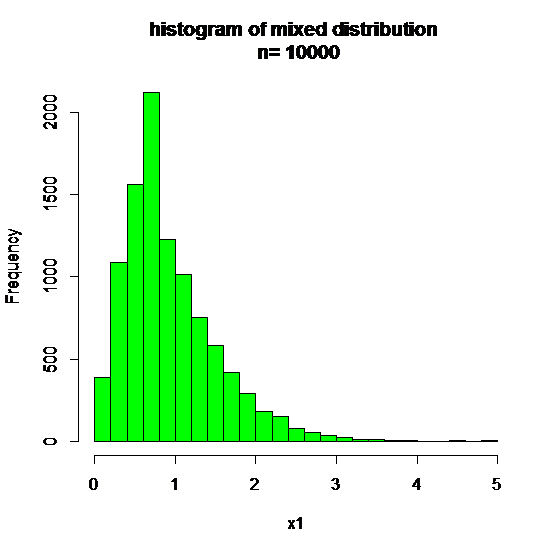
\includegraphics{q3_10000.png}}
		\caption{Graph of u(i) vs u(i-1) for $ N = 10000 $}	
		\label{3:q3_f1_c}
	\end{figure}
	


From the above graphs , it is easily understood that random numbers generated by the Linear Congruence Generator for $a = 1229,\: b = 1$ and $m = 2048$ lie on $5$ parallel lines. The slope ($m$) of the lines is given by:-
\begin{align}
m &= \frac{y_1 - y_0}{x_1 - x_0} \\
\intertext{Let us take the points to be on the 1$^{\textrm{st}}$ line for $N=1000$ . The start and end co-ordinates are $(0,\: 0)$ and $(1.0,\: 0.2)$ respectively.Therefore, the slope ($m$) of the line is :-}
m &= \frac{0.2 - 0}{1.0 - 0.0} = 0.2 \\
\intertext{Hence all the random numbers generated by the above sequence lie on lines with the following equation ($c$ being the y-intercept):-}
x - 5y + 5c &= 0
\end{align}

\subsubsection{R Code}
\lstinputlisting[caption={\texttt{R} code which generates the points for $(u_{i-1}, u_i$)}, label=lst:q3_prog1, language=R]{question3.R}
\subsection{Interpretation of results}
\begin{itemize}
\item As we increase $N$ we get more and more points on 5 parallel lines whose equation is given by  $x-5y+5c=0$ ($c$ being the y intercept.)
\item Changing the value of $x_0$ does not affect the graph and we get almost similar graph.
\end{itemize}

\end{document}
